\chapter{Event generation, simulation, reconstruction, and analysis software}
\label{chap:Reconstruction}

\chapterquote{When I walk along with two others, from at least one I will be able to learn.}%
{Confucius, 551 BC $-$ 479 BC}%: Blackwood's Magazine May 1830

%As previously stated, this document focus on the \ILD and \CLICILD detectors. Due to the similarity, we often only discuss one detector to avoid the repetition. The difference in detectors will be stated if applicable.

%In previous chapters, overviews of the particle physics theory and the detectors of the future linear collider experiments have been provided.


 %Automated analysis is the only way to deal with the vast amount of data generated in high energy physics. Hence the software supporting the automated analysis are important. An analysis often consists of  Monte Carlo event generation, event reconstruction, and using software to extract information of the event.
%  The software for the future linear colliders shares a  common software framework.

In this chapter, event generation. simulation, reconstruction, and analysis software for the future linear colliders  are discussed. The event reconstruction focuses on the \pandora event reconstruction, which is the framework for the photon reconstruction algorithms in \Chapter{chap:Photon}. The multivariate analysis (MVA) is discussed  in details due to its complexity.

\section{Event generation}
\label{sec:pandoraMC}

Monte Carlo (MC) samples were generated for physics analyses in this thesis. Most events used in this thesis were generated with the \WHIZARD software \cite{whizard,Moretti:2001zz}. Some simple events, such as single-photon-per-event samples, were generated by writing the event manually in the  HEPEVT format \cite{Altarelli:1989hx}. The \PYTHIA software \cite{Sjostrand:1995iq} was used to describe parton showering, hadronisation and fragmentation. The fragmentation parameters for the \PYTHIA were tuned to OPAL data \cite{Alexander:1995bk} from the Large Electron-Positron Collider (\LEP). The \TAUOLA software \cite{Jadach:1993hs} was used to describe the tau lepton decay with correct spin correlations of the tau decay products. The Initial State Radiation (\ISR) effect is simulated in the \WHIZARD, with the \ISR photons being collinear with the beam direction. The Final State Radiation (\FSR) is simulated in the \PYTHIA with default parameters.

Particle masses and widths used to generate SM samples for studies with \CLIC detectors, used in \Chapter{chap:DoubleHiggs}, are listed in \Table{tab:pandoraCLICparticleMass}.

\begin{table}[htbp]
\centering
\smallskip
\begin{tabular}{l r  r }
\hline
\hline
Particle &  Mass (\uprightMath{GeV/c^2}) & Width (\uprightMath{GeV/c^2}) \\
\hline
\Pup, \Pdown, \Pstrange quarks& 0 &  0\\
\Pcharm quark& 0.54 &  0\\
\Pbottom quark& 2.9 &  0\\
\Ptop quark& 174 & 1.37\\
\PW boson & 80.45 &  2.071\\
\PZ boson & 91.188 &  2.478\\
\hline
\hline
\end{tabular}
\caption[Masses of quarks and bosons used for  generating Standard Model samples.]%
{Particle masses and widths used for the generation of SM samples for \CLIC detectors, taken from \cite{Linssen:2012hp}. The Higgs boson mass is specified for individual samples.}
\label{tab:pandoraCLICparticleMass}
\end{table}
%, with no polarisation of the electron and positrons.



\subsection{\CLIC luminosity spectrum}
\label{sec:pandoraCLUClumi}

The electron$-$photon interaction, where the photon is produced from initial state radiation via Beamstrahlung,  has a different  instantaneous luminosity than the electron$-$positron interaction. Hence, for the same time period, the total integrated luminosities of the electron$-$photon and photon$-$photon interactions are different to that of the electron$-$positron interaction.

As all events were generated assuming a total integrated luminosity of the   electron$-$positron interaction, a correction in the total integrated luminosity  is needed for  electron-photon and photon-photon interactions where the photon is produced from initial state radiation via Beamstrahlung.

A simulated study \cite{Sailer:lumi} was performed to identify the ratios of the integrated luminosities of the  positron$-$photon, electron$-$photon, and photon$-$photon interactions where  initial-state photons are from Beamstrahlung,   to the electron$-$positron interaction at \CLIC. Results of the study is  summarised in \Table{tab:reconstrcutionBSlumi}. For the physics analysis in \Chapter{chap:DoubleHiggs}, integrated luminosities  for processes with initial-state photons from Beamstrahlung are corrected with the values in \Table{tab:reconstrcutionBSlumi}.
% with the GUINEAPIG \cite{Schulte:1999tx} and was simulated in the \WHIZARD
\begin{table}[htbp]
\centering
\smallskip
\begin{tabular}{l r  r }
\hline
\hline
Luminosity ratio &  \rootS{1.4} & \rootS{3} \\
\hline
L(\ee) / L(\ee) &1 & 1\\
L(\HepProcess{\Pep\Pgamma}) / L(\ee) &0.75 & 0.79\\
L(\HepProcess{\Pem\Pgamma}) / L(\ee) &0.75 & 0.79\\
L(\Gammagamma) / L(\ee) &0.64 & 0.69\\
\hline
\hline
\end{tabular}
\caption[Luminosity ratio for processes with initial-state photons from Beamstrahlung.]%
{Luminosity ratios of total integrated luminosities of the  positron$-$photon, electron$-$photon, and photon$-$photon interactions  where initial-state photons are from Beamstrahlung,  to the electron$-$positron interaction, for \CLIC, at \rootS{1.4} and 3\,TeV. Values are taken from \cite{Sailer:lumi}.}
\label{tab:reconstrcutionBSlumi}
\end{table}

\section{Event Simulation}


%For all the simulated events used in this thesis, t

The simulation software used to simulate the interaction of particles through the detector material is the \GEANT software \cite{Agostinelli:2002hh}. The \ILD and \CLICILD detector geometry descriptions are provided by the \Mokka software \cite{MoradeFreitas:2002kj}.  The QGSP\_BERT physics list from \GEANT the  is used to simulate the detailed development of hadronic showers in the detector. Since events were generated with head-on collisions, the event simulation introduced the crossing angles (20\,mrad for \CLIC and 14\,mrad for \ILC) by applying a corresponding Lorentz boost to all particles in the events.

%The  QGSP\_BERT physics list uses the Bertini model \cite{Proceedings:2003lxa} at low energies, making a transition to the Low Energy Parameterisations (GHEISHA \cite{TechnicalReportPITHA 85-02}) model between 9.5 and 9.9\,GeV, and a further transition to the QGSP model between 12 and 25\,GeV.  QGSP model is a GEANT4 implementation of a string model~\cite PhysRevLett.67.1523 for the high energy interaction, supplemented by the  GEANT4} precompound model\cite{mazzucato2001proceedings}
%QGSP is the basic physics list applying the quark gluon string model for high energy interactions of protons, neutrons, pions, and Kaons and nuclei. The high energy interaction creates an exited nucleus, which is passed to the precompound model modeling the nuclear de-excitation.
%QGSP_BERT and QGSP_BERT_EMV
%Like QGSP, but using Geant4 Bertini cascade for primary protons, neutrons, pions and Kaons below ~10GeV. In comparison to experimental data we find improved agreement to data compared to QGSP which uses the low energy parameterised (LEP) model for all particles at these energies. The Bertini model produces more secondary neutrons and protons than the LEP model, yielding a better agreement to experimental data.

\subsection{\CLIC beam induced backgrounds}
\label{sec:pandoraggHad}

It is necessary to include beam induced background to study \CLIC detectors under realistic conditions. Two most significant types of backgrounds  \cite{Linssen:2012hp} in the \CLIC colliding environment are \ggHad and incoherent \ee pairs. The \ggHad background is produced when the interaction of real and virtual beamstrahlung photons from the colliding beams leads to two-photon interactions, resulting in  hadronic final states \cite{Drees:1991zka, Chen:1993dba}. The incoherent \ee pairs are produced with interactions of both real or virtual beamstrahlung photons with individual particles of the other beam, producing \ee pairs in the strong electromagnetic fields \cite{Chen:1992ax}.

%One issue to consider when studying   the \CLICILD detector concept is the beam induced background.

\TABLE{tab:reconstrcutionBackgroundEnergy} shows the amount of energies deposited from \ggHad and the incoherent pairs in different parts of the \CLICILD detector. The energies in the calorimeter are integrated over 300\,ns from the start of the bunch train. The \ggHad is the dominant background in all calorimeters except the \HCAL endcap. For the study presented in \Chapter{chap:DoubleHiggs}, only the \ggHad background is included in the simulation.


\begin{table}[htbp]
\centering
\smallskip
\begin{tabular}{l r  r }
\hline
\hline
Subdetector &  Incoherent Pairs (TeV) & \ggHad (TeV) \\
\hline
\ECAL Endcaps & 2 & 11\\
\ECAL Barrel & - & 1.5\\
\HCAL Endcaps & 16 & 6\\
\HCAL Barrel & - & 0.3\\
\hline
Total Calorimeter & 18 & 19 \\
\hline
Central Tracker & - & 7 \\
\hline
\hline
\end{tabular}
\caption
{Amount of energies deposited from \ggHad and the incoherent pairs in the different parts of the \CLICILD subdetectors. Numbers correspond to the background for an entire \CLIC bunch train and were obtained for nominal background rates. The reconstructed calorimeter energies are integrated over 300\,ns from the start of the bunch train. The table is adapted from \cite{Linssen:2012hp}.}
\label{tab:reconstrcutionBackgroundEnergy}
\end{table}

The simulation of \ggHad uses the photon spectrum from \Guineapig \cite{Schulte:1999tx} and a parametrisation of the total cross section of the \ggHad process  based on \cite{Schuler:1996en}. The average number of \ggHad events per bunch crossing within the detector acceptance at \rootS{3} is 3.2, for a \Gammagamma centre-of-mass energy greater than 2\,GeV  \cite{Barklow:1443518}. The \PYTHIA software is used to simulate the hard interaction and the hadronisation of these \ggHad events.


The hits from simulated \ggHad events were superimposed to simulated \ee, \Egamma, and \Gammagamma collisions before the event reconstruction. The \ggHad backgrounds included are resulted from 60 bunch crossings, corresponding to a time window of $-5$\,ns to $+25$\,ns around the generated physics event, with a 0.5\,ns timing separation between bunch crossings to mimic the \CLIC train structure \cite{Linssen:2012hp}. For each bunch crossing, the number of \ggHad events superimposed were chosen from a Poisson distribution with a mean of 3.2.


\section{Event Reconstruction}

% as a part of the \ilcsoft software package
Reconstruction software runs in the \Marlin framework \cite{Gaede:2006pj}. The event reconstruction contains following steps: digitisation of simulated calorimeter hits, reconstruction of tracks in the tracking system (using pattern recognition algorithms) \cite{Gaede:2014aza}, and particle flow objects (\PFOs) reconstruction with \pandora\cite{Thomson:2009rp,Marshall:2012ry}.

% Details of the event reconstruction can be found in \cite{Brau:2007zza,Linssen:2012hp}.

Different \Marlin processors are used to reconstruct tracks: ClupatraProcessor \cite{Gaede:2014aza} for tracks in the \TPC, ForwardTrackingProcessor \cite{Gaede:2014aza} for tracks in the \FTD, and SiliconTrackingProcessor \cite{Gaede:2014aza} for tracks in other silicon tracking detectors. A final \Marlin tracking processor, FullLDCTrackingProcessor \cite{Gaede:2014aza}, is used to combine tracks segments produced from individual processors.

%Tracks in the TPC are reconstructed with a \Marlin processor, ClupatraProcessor \cite{Gaede:2014aza}. Tracks in the \FTD are reconstructed with the ForwardTrackingProcessor \cite{Gaede:2014aza}. The reconstruction of tracks other silicon tracking detectors are performed with the SiliconTrackingProcessor \cite{Gaede:2014aza}. The final combination of the TPC, \FTD, and silicon tracks are done in  the FullLDCTrackingProcessor\cite{Gaede:2014aza}.

%Here particle flow reconstruction via \pandora will be discussed in details, as \pandora provides the software framework for the photon reconstruction in \Chapter{chap:Photon}. The \pandora event reconstruction is also used in the analyses in  \Chapter{chap:Tau} and \Chapter{chap:DoubleHiggs}.

\subsection{\pandora event reconstruction}
\label{sec:pandoraPandoraPFA}

%The tradition energy flow approach to calorimetry is unable to meet the mass and energy resolution requirements for future linear colliders. The particle flow approach to calorimetry with \pandora has a proof-of-principle demonstration of its capability to reach the required jet energy resolution. The particle flow approach to calorimetry  also puts stringent requirements on the detector design, which is described in \Section{sec:detectorPhysicsRequirementPandora}. By associating calorimeter hits to the tracks, around 60\% of the jet energy from charged particles is measured by the tracking detector, which has a much better resolution than the calorimeter. Small cell sizes of the calorimeters are required to identify calorimeter hits from different particles. The traditional sum of calorimeter cell energies is hence replaced by particle flow reconstruction algorithms - a complex pattern recognition problem.

%The \pandora algorithm has been developed and used in the \ILC and \CLIC simulation studies.
The \pandora event reconstruction is used in the studies for future \ee linear colliders. Originally developed with the \ILD detector concept \cite{Thomson:2009rp}, \pandora has been adapted to the \CLIC condition and shows its ability to deliver required energy resolutions \cite{Linssen:2012hp,Marshall:2012ry}. There are over 60 \ee linear collider specific reconstruction algorithms. Each algorithm aims to address a particular topological issue in the reconstruction. In the recent development, the core base codes for basic objects and memory managements were factorised into the Pandora C++ Software Development Kit \cite{Marshall:2015rfa}.
% Recent the code base of the \pandora has been restructured.

In the subsequent sections, the main steps in the \pandora reconstructions are summarised. The details of the \pandora event reconstruction can be found in \cite{Thomson:2009rp,Marshall:2012ry,Marshall:2015rfa}.  The inputs of the \pandora event reconstruction are digitised calorimeter hits and reconstructed tracks, with some detector information, such as magnetic field strength, to aid the reconstruction. The output are reconstructed Particle Flow Objects (\PFOs).

\subsubsection{Track processing}
\label{sec:pandoraPandoraTrack}


Tracks from the inner tracking detectors are important inputs for the \pandora reconstruction.  A helical track fit using last 50 reconstructed hits in the tracking detector is performed to project the track onto the front of the \ECAL. Afterwards,  special topologies of tracks are identified based on the  likely origin of the track.  The topologies of tracks include when a neutral particle decays or converts into a pair of charged tracks, leaving tracks of a ``V0''  shape. This is identified by searching for a pair of tracks originated from a single point. Another topology is the ``kinks'' when a charged particle decays to a single charged particles with neutral particles. The   topology of  the ``prongs'' is also identified when a charged particle decays to multiple charged particles. This information about special topologies, along side with helical track fit, the track projection onto the front of the \ECAL, and the original track parameters, is stored and passed onto the subsequent reconstruction.

%Tracks from the inner tracking detectors are important inputs for the \pandora reconstruction. These tracks are selected based on their topological properties, how likely they are from physical processes, and whether they are consistent with the tracker resolution. Only tracks passing the selection are used for the subsequent reconstruction.

%This information about special topologies of tracks, along side with helical track fit (using last 50 reconstructed hits in the tracking detector) and the track projection to the front of the \ECAL, is stored and passed onto the subsequent reconstruction. Identified special topologies of tracks include when a neutral particle decays or converts into a pair of charged tracks, leaving tracks of a ``V0''  shape. This is identified by searching for a pair of tracks originated from a single point. Another topology is the ``kinks'' when a charged particle decays to a single charged particles with neutral particles. The last special topology are  the ``prongs'' when a charged particle decays to multiple charged particles. This information about special topologies, along side with helical track fit (using last 50 reconstructed hits in the tracking detector) and the track projection to the front of the \ECAL, is stored and passed onto the subsequent reconstruction.

\subsubsection{Calorimeter hit processing}

The other important inputs of  the \pandora reconstruction are the calorimeter hits from calorimeters. The properties of a calorimeter hit and the extra calculated information about calorimeter hits are stored and used in later steps.  The properties of a calorimeter hit include its position, its layer in the calorimeter, and its energy response from the calorimeter digitiser. The extra calculated information about calorimeter hits  includes  likelihood of the hit originated from a minimum ionising particle (MIP).

%Calorimeter hits are selected based on a series of criterion. The selected hits need to have energies above certain thresholds, measured in minimum ionising particle (MIP) equivalent or measured in directly converted energy. Only calorimeter hits that pass the selection are used in later steps.

Isolated hits, often originated from low energy neutrons in a hadronic shower, can be at a significant distance from the point of the production. Therefore, they are of little use to the \pandora reconstruction as it is impossible to associate isolated hits to the correct hadronic shower. These hits are identified and not used during the clustering stage. However, these isolated hits participate in the reconstruction in the particle flow object (PFO) creation step to contribute to the energy estimation of the PFO.


\subsubsection{Particle Identification}
\label{sec:particleID}

Dedicated particle identification algorithms find calorimeter hits associated with neutral particles, such as muons and photons. These calorimeter hits associated with muons and photons are removed from the subsequent reconstruction for charged particles. Identified muons and photons  re-enter the reconstruction at the fragment removal stage (see \Section{sec:pandoraFragmentRemoval}).  \CHAPTER{chap:Photon} describes the photon reconstruction  algorithms in details.

%To improve the reconstruction of the charged particles which associates  calorimeter hits to tracks,

%As fewer hits are left to be reconstructed with charged particles, the reconstruction of charged particles is improved.
%do not participate in the later clustering and re-clustering stages, but
% and the pattern recognition problem is simplified.

%Dedicated particle identification algorithms aim to identify muons and photons before associating calorimeter hits to tracks.

\subsubsection{Clustering}
\label{sec:pandoraConeCluster}

Cone-based clustering algorithms are used to group calorimeter hits into clusters. The output \clusters are further processed, merged, or split based on their topological properties.

%Since the cone clustering algorithm is widely used in many other reconstruction algorithms in \pandora reconstruction, it is necessary to introduce the cone based clustering algorithm, before discussing the rest of the \pandora reconstruction.

Illustrated in \Figure{fig:pandoraConeClustering}, cone based clustering algorithm identifies a seed first, shown as the yellow dot. The algorithm then forms a cone to include hits that are within a specified opening angle to the direction of the cone. Afterwards the cone with the associated hits forms the cluster.

% The main type of clustering algorithms used in the  \pandora is the cone based algorithms. The direction of the seed is typically used as the   direction of the cone.

%these cone clusters have similar direction and energy to the originated particle. Therefore it is applicable to use cone based clustering algorithms for building clusters.

\begin{figure}[tbph]
\centering
{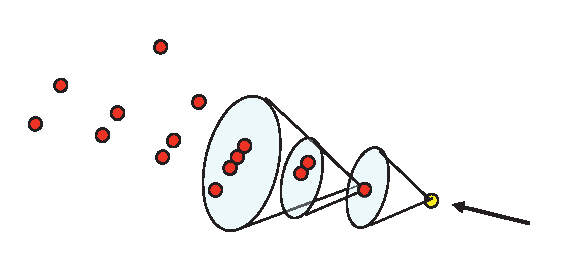
\includegraphics[width=0.5\textwidth]{pandora/coneClustering}}%
\caption{Illustration of the cone based clustering algorithm, taken from \cite{Marshall:pandoraLC}}
\label{fig:pandoraConeClustering}
\end{figure}

The cone-based clustering algorithm is used in \pandora reconstruction because the direction of the particle flow is largely unchanged from the originated particle, irrespective of  the particle flow being an electromagnetic shower, QCD radiation, or hadronisation. \FIGURE{fig:pandoraConeClustering2} illustrates the cone-based clustering algorithm used in the \pandora reconstruction. The seed for the cone clustering is typically the projection of a track onto the front of the \ECAL.  The initial cone direction is taken as the direction of the seed. Afterwards, a cone with a specified opening angle will be formed around the direction of the seed.

%and a cluster is formed with the calorimeter hits in the cone associated.

%A calorimeter hit can also be used as a seed.

The building of the cone is iterated from the inner layer of the \ECAL to the outer layer. At each layer, possible associations with calorimeters hits in previous layers and the same layer are made. If a calorimeter hit is not associated with the cone, the hit is used to seed a new cluster. %The clustering algorithm produces basic working objects, \clusters.

\begin{figure}[tbph]
\centering
{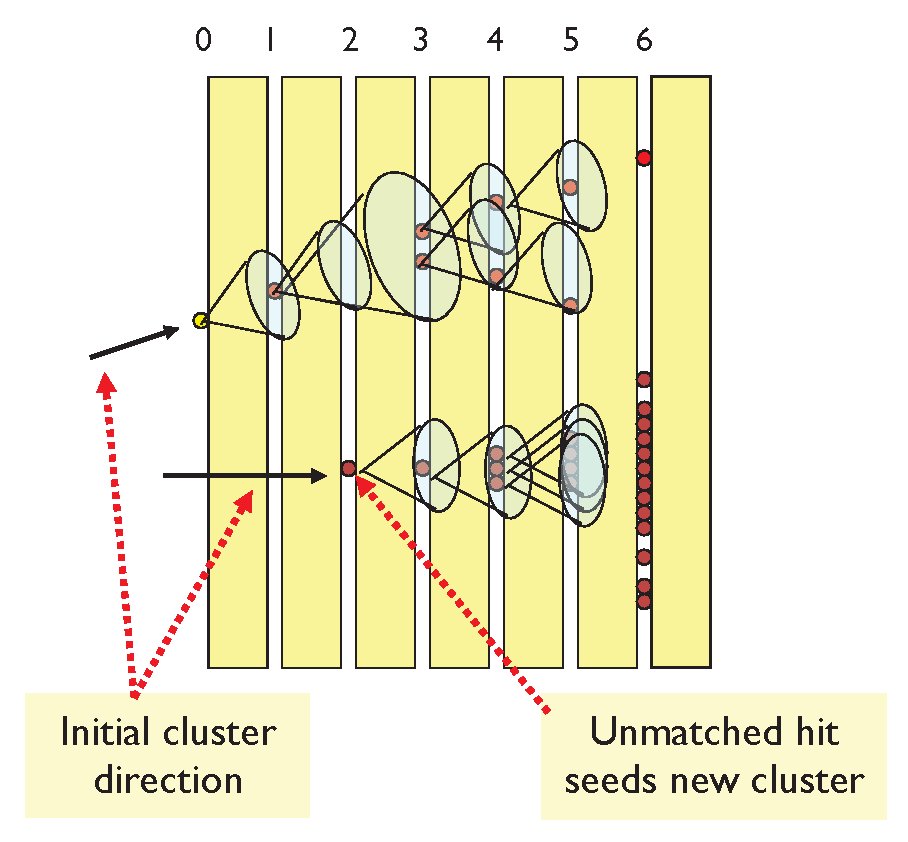
\includegraphics[width=0.5\textwidth]{pandora/coneClustering2}}%
\caption{Illustration of the clustering algorithm used  in the \pandora, taken from \cite{Marshall:pandoraLC}}
\label{fig:pandoraConeClustering2}
\end{figure}

\subsubsection{Topological cluster association}

After the initial clustering, clusters are further refined using topological information of calorimeter hits in the calorimeters. The initial clustering scheme tends to form small clusters. These small clusters are then merged  based on clear topological signatures. Main rules for topological association algorithms  are schematically shown in \Figure{fig:pandoraTopoAsso}. Some merging signatures include combining track segments, connecting track segments with gaps, connecting track segments to hadronic showers, and merging clusters when they are within close proximity.
%This step is necessary because t
%for looping track segments, back-scattered tracks from hadronic showers, and cone association are shown
% In each case, the arrow indicates the tracks. The dark red dots represent the calorimeter hits in the associated cluster. The slightly fainter red dots represent the calorimeter hits in the neutral cluster. The black line represents the front of the \ECAL.
\begin{figure}[tbph]
\centering
    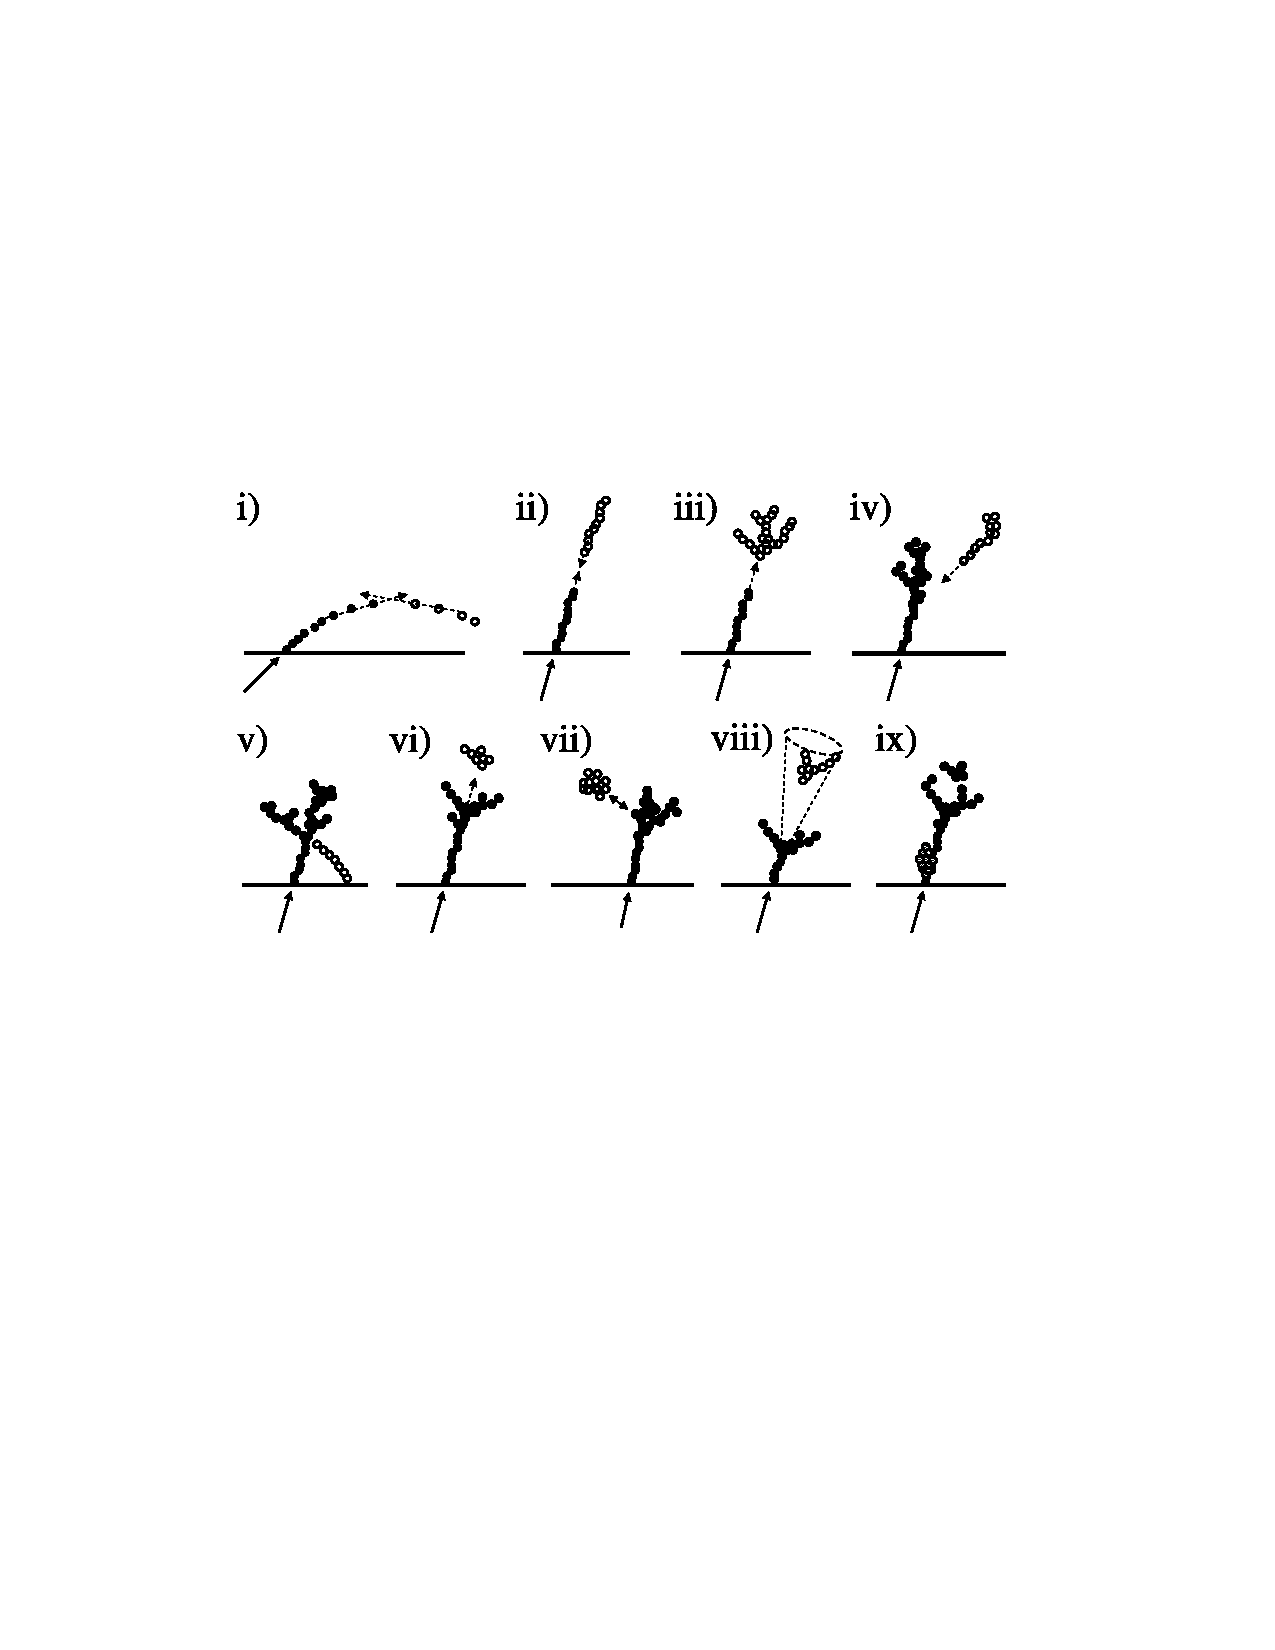
\includegraphics[width=0.85\textwidth]{pandora/topological}
\caption[Topological association in the \pandora.]
{The main topological rules for cluster merging:  i) looping track segments; ii) track segments with gaps; iii) track segments pointing to hadronic showers; iv) track-like neutral clusters pointing back to a hadronic shower; v) back-scattered tracks from hadronic showers; vi) neutral clusters which are close to a charged cluster; vii) a neutral cluster near to a charged cluster; viii) cone association; and ix) recovery of photons which overlap with a track segment. In each case the arrow indicates the track, the filled points represent the hits in the associated cluster and the open points represent the hits in the neutral cluster. Figures are taken from \cite{Thomson:2009rp}.}
\label{fig:pandoraTopoAsso}
\end{figure}

\subsubsection{Track$-$cluster association}

Having refined the clusters in the calorimeter, the next step is to associate the clusters to the tracks obtained from the inner tracking detectors. The associations  are made according to the proximity of the first layer of the cluster and the track projection onto the front of the \ECAL, whilst demanding a  match between the track direction and the initial cluster direction, and a match between the track momentum and the cluster energy.

%A match between the track direction and the initial cluster direction, as well as a match between the track momentum and the cluster energy, are required for the track$-$cluster association.


\subsubsection{Re-clustering}

The track$-$cluster association scheme described in the previous section works well for events with jets of less than 50\,GeV energies. In a dense jet environment with  higher energy jets, electromagnetic and  hadronic showers are  boosted and are likely to overlap each other. Therefore, it is important to refine the track-cluster association based on the information from the momentum of the track and the energy of the cluster.

The re-clustering stage improves the compatibility of the cluster energy and the associated track momentum. It is performed on a statistical basis. If mismatch between  the cluster energy and the associated track momentum is identified, the cluster will be re-clustered either using the same clustering algorithm with different parameters, or different clustering algorithms. This re-clustering step creates many temporary clusters. Out of many temporary clusters, the temporary cluster with the best track$-$momentum cluster$-$energy match is chosen, and that cluster is  associated with the track.


A schematic diagram of the re-clustering stage is shown in \Figure{fig:pandoraRecluster}.  In this example, the initial cluster energy is less than the associated track momentum. The topological association algorithms did not add the natural cluster, as it would have formed a cluster with too much energy. The re-clustering scheme tries different cone clustering algorithms by splitting the neutral cluster so that the topological association could make a correct association of the cluster to track.

%In the figure, the black upright arrows indicate the tracks. The dark red dots represent the calorimeter hits in the associated cluster. The  slightly fainter red  dots represent the calorimeter hits in the neutral cluster.

\begin{figure}[tbph]
\centering
{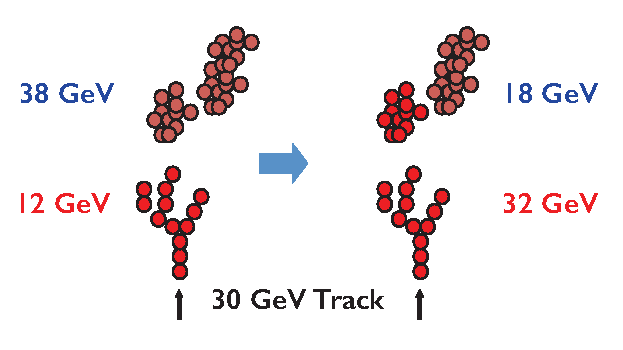
\includegraphics[width=0.6\textwidth]{pandora/recluster}}%
\caption[Illustration of the re-clustering algorithm in \pandora]
{Illustration of the re-clustering algorithm in \pandora, taken from \cite{Marshall:pandoraLC}. Arrows indicate the tracks. Dark red dots represent the calorimeter hits in the associated cluster. Slightly fainter red  dots represent the calorimeter hits in the neutral cluster. The initial cluster energy is less than the associated track momentum. The topological association algorithms did not add the natural cluster, as it would have formed a cluster with too much energy. The re-clustering algorithm tries different cone clustering algorithms to split the neutral cluster so that the topological association could make a correct association.}
\label{fig:pandoraRecluster}
\end{figure}

\begin{comment}
\subsection{Photon identification}

The neutral clusters are tested against an expected photon electromagnetic shower profile. The longitudinal shower profile for a photon cluster is required to be similar to a expected electromagnetic shower profile, with the discrepancy being smaller than a threshold.
\end{comment}

\subsubsection{Fragment removal}
\label{sec:pandoraFragmentRemoval}

This stage of the \pandora reconstruction will focus on merging clusters that are likely to be fragments of other particles. Typically a fragment is merged if it is close to the parent cluster and the fragment has a low energy.  Algorithms for photon fragment merging  are described in details in \Chapter{chap:Photon}.

 %The merging criterion are mostly based on the proximity of the fragment to the particle, and the energy comparison of the fragment to the particle.

\subsubsection{Particle Flow Object Creation}
\label{sec:pandoraPFOcreation}

% double counting taking care in pandora
The last stage of the reconstruction is to create the output objects, Particle Flow Objects (PFOs). The PFOs contain clusters and associated tracks and calorimeter hits. Particle identification for electrons, muons, and photons are applied to \PFOs.

%The output objects, \PFOs, contain information of positions, four-momenta, particle ID, and other quantities. These \PFOs are heavily used  in physics analyses.

% The electron, muon and photon identifications associated with the \PFOs are  also used in physics analyses, for example, the analyses in \Chapter{chap:Tau} and in \Chapter{chap:DoubleHiggs}.


\subsection{\CLIC beam induced backgrounds suppression}

%There are a few  simulation and reconstruction issues specific to the \CLIC, which affect the analysis in \Chapter{chap:DoubleHiggs}. One issue is that the luminosity spectrum for  interactions with photon from Beamstrahlung is different to the luminosity spectrum of electron-positron interactions. A solution is presented in \Section{sec:pandoraCLUClumi} to correct for the differences. Another issue is that there is a large amount of beam induced background in the \CLIC environment, which needs to be suppressed before physics analyses. The background suppression is described in \Section{sec:pandoraggHad}. Lastly simulated masses of particles are given in \Section{sec:pandoraCLICsimMass}.

%One issue is that the event reconstruction does not include calorimeters hits in the forward calorimeters due to computational reasons. Instead, a fast simulation using MC particles is used and details are laid out in \Section{sec:doubleHiggsForwardElectron}.


Following the discussion on \CLIC beam induced background,  two software have been developed to suppress \ggHad backgrounds: a track selector and a PFO selector \cite{Marshall:2012ry}.

The track selector, CLICTrackSelector processor \cite{Marshall:2012ry},  removes poor quality and fake tracks that are  likely from the beam induced background. It examines the number of track hits in individual tracking subdetectors and places a track-quality cut. It also places a cut on the arrival time of the track onto the front of the \ECAL. If the arrival time of the track at the front of the \ECAL using the helical fit of the track differs more than 50\,ns from using a straight line fit, the track will be rejected.


The PFO selector \cite{Marshall:2012ry} discards PFOs that are originated from the beam induced background from the event reconstruction, based on the transverse momentum (\pT) and time information of the PFOs. The PFOs from \ggHad often have low \pT and are distributed in time across the reconstruction integration timing window. In contrast, the PFOs from physics processes have a range of \pT, and have times close to the time of the brunch crossing that contains the physics event.

%By utilising the high spatial resolution from the high granular calorimeter, individual PFOs can be tracked and reconstructed.

For the best performance of the background suppression, the PFO selector uses different \pT and timing cuts for the central part of the detector and for the forward part of the detector. The PFO selector also uses different \pT and timing cuts for different types of particles: photons, neutral PFOs, and charged PFOs.

Three configurations of these cuts are developed: ``loose'', ``normal'', and ``tight'' PFO selections. As the name suggested, ``loose'' PFO selection corresponds to a looser cut of \pT and time, preserving PFOs with a larger range of \pT and a larger range of  times than the ``tight'' PFO selection.

The optimal configuration of the PFO selection to suppress the backgrounds depends on the centre-of-mass energy of the collision and the physics process to study. \FIGURE{fig:pandoraEvtDisplayggHad} shows the effect of the suppression of the background with the tight \PFO selection.  \FIGURE{fig:pandoraEvtDisplayggHad1} shows reconstructed particles  in a simulated \HepProcess{\Pep\Pem \to \PHiggs\PHiggs \to \Ptop\APbottom\Pbottom\APtop} event which are integrated over a time window of 10\,ns (100\,ns in \HCAL barrel) in the \CLICILD detector model, with 60 bunch crossings of \ggHad background overlaid. The effect of applying tight \PFO selection cuts is shown in \Figure{fig:pandoraEvtDisplayggHad2}. The energy deposited in the detector by the background is reduced from 1.2\,TeV to the level of 100\,GeV.


\begin{figure}[tbph]
\centering
  \begin{subfigure}[b]{0.45\textwidth}
    \includegraphics[width=\textwidth]{pandora/evtDisplayggHad1.eps}
    \caption{}
    \label{fig:pandoraEvtDisplayggHad1}
  \end{subfigure}
  \begin{subfigure}[b]{0.45\textwidth}
    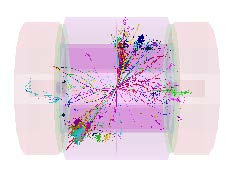
\includegraphics[width=\textwidth]{pandora/evtDisplayggHad2.eps}
    \caption{}
    \label{fig:pandoraEvtDisplayggHad2}
  \end{subfigure}
\caption[Effect of the suppression of the background with the tight \PFO selection.]
{Reconstructed particles  in a simulated \HepProcess{\Pep\Pem \to \PHiggs\PHiggs \to \Ptop\APbottom\Pbottom\APtop}  are integrated over a time window of 10\,ns (100 \,ns in \HCAL barrel) event in the \CLICILD detector model, with 60 bunch crossings of \ggHad background overlaid in \Figure{fig:pandoraEvtDisplayggHad1}. The effect of applying tight \PFO section cuts is shown in \Figure{fig:pandoraEvtDisplayggHad2}. The energy deposited in the detector by the background is reduced from 1.2\,TeV to the level of 100\,GeV. Figures are taken from \cite{Marshall:2012ry}.}
\label{fig:pandoraEvtDisplayggHad}
\end{figure}



\section{Analysis software}

%In the previous sections the automated reconstruction tools are described in details. This section is dedicated to the analysis software, which will be used in the analyses described in subsequent chapters.

\subsection{Monte Carlo truth linker}
\label{sec:pandoraMCtruthLink}
It is extremely useful to be able to associate reconstructed objects to the Monte Carlo particles, for algorithms development and  event selection optimisation. The MC truth linker processor provides the link between a MC particle and a  reconstructed calorimeter hit. From the link, the MC particle contributing most to a reconstructed \PFO or a group of \PFOs (a jet) can be determined.

\subsection{Jet algorithms}
\label{sec:pandoraJetAlg}

%For the linear collider, thanks to the high granular calorimeter and advanced PFA software, the starting point for analysis are individual Particle Flow Objects (PFOs), as well as individual tracks. Each of the PFOs encodes four-momentum and position information. At the same time, tracks would have momentum and position information.

It is useful to group PFOs and tracks into jets, which are the results of hadronisation processes from high energy particles like quarks or gulons. A jet is typically a visually obvious structure in an event display. The momentum and the direction of a jet tend to resemble the original particle. Despite the relative simplicity of identifying jets visually, it is a challenge for a pattern recognition program to identify jets effectively and efficiently. Early work on jet finding started in 1977 \cite{Sterman:1977wj}, where descriptions on later developments can be found in reviews \cite{Moretti:1998qx,Salam:2009jx,Ali:2010tw}.

There are two large families of jet finding algorithm: cone based algorithms, and sequential combination algorithms. The cone based algorithms are briefly discussed in \Section{sec:pandoraConeCluster} in the context of the \pandora reconstruction. Here the focus is on the sequential combination algorithms.

Sequential combination algorithms typically calculate a pair-wise distance metric between a seed and a particle. The particle with the smallest metric is combined with the seed and  into the jet. The distance metric will be updated after a combination. This procedure is repeated until some stopping criterion are satisfied. The different jet algorithms typically differ in the definitions of  distance metrics and stopping criterion.
%, and a pair with smallest metric will be combined.

The chosen jet algorithm implementation used in this thesis is the FastJet C++ software package \cite{Cacciari:2011ma,Cacciari:2005hq}. The notations in the subsequent discussion follow the convention in \cite{Cacciari:2011ma}.

% The implementation in the \Marlin software package is called the MarlinFastJet. The package provides a range of jet finding algorithms.

\subsubsection{Longitudinally invariant \kt algorithm}

Longitudinally invariant \kt algorithm \cite{Catani:1993hr,Ellis:1993tq} is one of the common sequential combination algorithms used in the \pp collider experiments. There are two variants of the algorithm: inclusive and exclusive. In the inclusive variant, the symmetrical pair-wise distance metric between particle $i$ and $j$, $d_{ij}$ or $d_{ji}$, and the beam distance, $d_{iB}$, are defined as
\begin{equation}
d_{ij}  & = d_{ji} = \min\!\parenths{\pT_{i}^{2},\!\pT_{j}^{2}}\frac{\DeltaOf{R_{ij}^{2}}}{R^{2}}, \\
d_{iB} & = \pT_{i}^2,
\end{equation}
where $\pT_{i}$ is the transverse momentum of particle $i$ with respect to the beam ($z$) direction, and $\DeltaOf{R_{ij}^{2}}$ is the measurement of angular separation of particle $i$ and $j$, defined as $\DeltaOf{R_{ij}^{2}} = \parenths{y_i - y_j}^2 + \parenths{\phi_i - \phi_j}^2$, where $y_i = \frac{1}{2}\ln\!\frac{E_i + {p_z}_i}{E_i - {p_z}_i}$ and $\phi_i$ are particle $i$'s rapidity and azimuthal angle. The free parameter $R$ controls the jet radius.

The $d_{ij}$ and $d_{iB}$ are calculated for all pairs of particles. If the minimum value of all $d_{ij}$ and $d_{iB}$ is a $d_{ij}$, particle $i$ and $j$ are merged and the four momentum of particle $i$ is updated as the sum of the two particles. If the minimum value is  a $d_{iB}$, particle $i$ is set to be a final jet and removed from the list of particles. The above procedure is repeated until no particles are left.


%If $d_{ij} < d_{iB}$, particle $i$ and $j$ are merged and the four momentum of particle $i$ is updated as the sum of the two particles.  Otherwise if $d_{ij} \geqslant d_{iB}$, particle $i$ is set to be a final jet. Particle $j$ is then used to seed a new jet. The above procedure is repeated until no particles are left.

%\fourMomentum of particle $i$ is updated as the sum of the two particles.

The exclusive variant is similar to the inclusive variant. First difference is that when the minimum value is  a $d_{iB}$, particle $i$ forms part of the beam jet. The beam jet contains particles that are considered to be from the beam induced background and discarded at the end of the jet clustering. The second difference is that when all $d_{ij}$ and $d_{iB}$ are above a threshold, $d_{cut}$, the jet clustering will stop.

The exclusive mode allows a specified number of jets to be found, where the $d_{cut}$ is automatically determined. In contrast, the inclusive mode would find as many jets as the algorithm allows.

%An example usage of the exclusive \kt algorithm can be found in \Section{sec:doubleHiggsJetOptimisation}.

\subsubsection{Durham algorithm}
\label{sec:pandoraJetDurham}
The Durham algorithm \cite{Catani:1991hj}, also known as \ee \kt algorithm, is commonly used in the \ee collider experiments. It only has one pair-wise distance metric:
\begin{equation}
d_{ij} = 2\min\!\parenths{E_i^2,\!E_j^2}\!\parenths{1 - \cosOf{\theta_{ij}}},
\end{equation}
where $E_i$ is the energy of particle $i$ and $\theta_{ij}$ is the angle between particle $i$ and $j$. The Durham algorithm can only be run at exclusive mode, which means that the clustering will stop when $d_{ij}$ is above a threshold, $d_{cut}$.

Compared to the longitudinally invariant \kt algorithm, the Durham algorithm uses energy instead of \pT in the distance metric, and it does not use the beam distance. This is because that for the \ee collider at low centre-of-mass energies, the beam induced background is not significant. And the total energy of the event is known, which is the same as the collision energy (for events with missing momentum).



\subsubsection{Jet algorithm for \CLIC}

Although \CLIC is a \ee collider, the  beam-induced background is significant and deposits a large amount of energy in the detector. Therefore, traditional \ee jet algorithms, like the Durham algorithm, are not suitable for the \CLIC colliding environment. Studies \cite{Linssen:2012hp,LCD-Note-2010-006} have shown that jet algorithms for the \pp colliders give better performances for the \CLIC  colliding environment. Therefore, longitudinally invariant \kt algorithm is often used in analyses with the \CLIC environment.

%A more recent attempt at marrying merits from both the Durham and the \kt algorithms has resulted in the Valencia jet algorithm \cite{Boronat:2014hva}. It has shown promising improvement compared to the \kt algorithm.

%, which is used in the parallel  \eeToHHbbbb  sub-channel analysis in \Chapter{chap:DoubleHiggs} by collaborators.


%Why extra C++ implementation speed reduce O(n^3) to NlgN y, phi space, 2D KNN problem

\subsubsection{The \y{} parameter}
\label{sec:pandoraYparameter}
The \y{} parameter is a measure of the number of jets in an event.  It describes the transition of  going from $N$ clustered jets to $N\!+\!1$ clustered jets using an exclusive jet algorithm. For example, $\y{23}$ would be the $d_{cut}$ value for an exclusive jet algorithm, above which the jet algorithm returns 2 jets, below which the jet algorithm returns 3 jets. Numerically the \y{} parameter is often much smaller than 1. A typically way to convert a small number to a machine acceptable range is to take  negative logarithm of the number.

\begin{comment}
\subsection{The \lcfiplus}
\label{sec:pandoraLCFI}
Another useful analysis technique is to identify jets from \Pbottom and \Pcharm quarks. These jets have signatory topologies. A combination of vertex finding and multivariate analysis is used to identify \Pbottom and \Pcharm jets.

The flavour tagging processor, \lcfiplus \cite{Suehara:2015ura} is based on the LCFIVertex package \cite{Bailey:2009ui}, which was used in the simulation studies for the \ILCloi \cite{Abe:2010aa,Aihara:2009ad} and the \CLICcdr \cite{Linssen:2012hp}.  The current software is modular and can be used in any order. However here it will be described in the order used in a physics analysis.

%The current software is built for a future \ee collider.

The inputs are \PFOs. The vertex finding algorithms perform vertex fitting and identify primary and secondary vertices. There is a ``V0'' particle rejection step in which neutral particles decay into pairs of charged particles. The topology is similar to the decay of \Pbottom or \Pcharm hadrons. Hence it is important to remove the V0 particles to improve the heavy quark flavour tagging (see \Section{sec:pandoraPandoraTrack} for a similar V0 rejection).

Once the primary and secondary vertices are found, \PFOs are clustered in to jets. This jet clustering scheme ensures that the secondary vertices and the muons, identified from semi-leptonic decay, fall into the same jet. Therefore, it is consistent with  hadronic decay. The jet algorithms used are Durham and Durham modified algorithms(see \Section{sec:pandoraJetDurham}).

The next step is to refine vertices to improve the \Pbottom jet identification from the \Pcharm jet. Since the existence of two close by vertices is strongly correlated to a \Pbottom jet, the vertices refining step will reconstruct as many secondary vertices correctly as possible.

The last step is to gather the information about vertices and jets, and deploy a multivariate analysis. The multivariate classier used, Boosted Decision Tree,  is implemented in the TMVA software package \cite{Hocker:2007ht}. A series of flavour sensitive variables are calculated, and the classification is divided into four subset: jets with zero, one, or two properly reconstructed vertices, or a single-track pseudo-vertex. For each subset, a jet can either be classified to a \Pbottom jet, a \Pcharm jet, or a light flavour quark jet (\Pup, \Pdown or \Pstrange). The \multiclass classifier's response is normalised across different subset, and they will be referred in the subsequent physics analysis as the tag value.

%The samples for training the \multiclass classifier are \HepProcess{\Pep \Pem \to \PZ \APnu \Pnu} at \rootS{1.4}, where \PZ decays to \HepProcess{\Pbottom\APbottom}, \HepProcess{\Pcharm\APcharm}, or \HepProcess{\Pup\APup/\Pdown\APdown/\Pstrange\APstrange}.

The flavour tagging is performed after the initial jet reconstruction, and all the \PFOs in the reconstructed jets are input into the \lcfiplus flavour tagging processor. Therefore, the classifier in the \lcfiplus processor is trained for a specific \PFO collection and a specific jet reconstruction algorithm. The outputs of the processor for a jet are three values, corresponding to the likelihood of the jet being a \Pbottom jet, a \Pcharm jet, or a light flavour quark jet.

%In this analysis, the classifier is trained with the optimal jet reinstruction choice, discussed in \Section{sec:doubleHiggsJetOptimisation}.
 % The selection efficiency of b-jets and c-jets with training samples is shown in \Figure{fig:doubleHiggs1.4Btag}.
\end{comment}


%\subsection{Event shape variables}
%\label{sec:pandoraEvtShape}
% ATTN used in tau chapter
\begin{comment}
Event shape variables are some useful global variables to describe the shape of the event, for example whether it is back-to-back, or homogenous in the solid angle.

The classical event shape thrust\cite{PhysRevLett.39.1587}, is defined as
\begin{equation}
T = \max_{\hat{t}}\!\frac{\sum_{i}\absOf{\hat{t}\!\cdot\!\vec{p_{i}}}}{\sum_{i}\absOf{\vec{p_{i}}}}
\end{equation}
where $\vec{p_{i}}$ is the momentum vector of the particle $i$. Summation is over all particles in the event. Thrust axis, $\hat{t}$, is a unit vector. (Principle) Thrust value, $T$, is 1 for a perfect pencillike back-to-back two-jet event, and 0.5 for a perfect spherical event. The thrust value is useful in picking out back-to-back two-jet event. Thrust axis is useful to separate each jet in a back-to-back two-jet event.
\end{comment}
\begin{comment}
A related variable , sphericity is  derived from the sphericity tensor \cite{PhysRevLett.35.1609}. The sphericity tensor is  defined as
\begin{equation}
\bm{S^{\alpha\beta}} = \frac{\sum_{i}p^{\alpha}_{i}p^{\beta}_{i}}{\sum_{i}\absOf{\vec{p_{i}}}^2},
\end{equation}
where $\vec{p_{i}}$ is the momentum vector of the particle $i$. Summation is over all particles in the event. $\alpha$ and $\beta$ refer to the x, y, z coordinate axis. Eigenvalues of tensor $\bm{S}$ can be found, or in this case diagonalisation of the matrix $\bm{S}$, denoted with $\lambda_{1}$, $\lambda_{2}$, $\lambda_{3}$. The normalisation condition requires $\lambda_{1}\!\geqslant\! \lambda_{2} \! \geqslant \! \lambda_{3}$ and $ \lambda_{1} \! + \! \lambda_{2} \! + \! \lambda_{3} \! = \! 1 $. Sphericity, $S$, is defined in terms of $\lambda$,
\begin{equation}
\sphericity = \frac{3}{2}\parenths{\lambda_{1} \! + \! \lambda_{2}}.
\end{equation}
\sphericity, is 0 for a perfect pencil-like back-to-back two-jet event, and 1 for a perfect spherically symmetric event.

Aplanarity is another useful event shape variable that distinguishes spherical symmetrical events from planar and linear events. The definition is
\begin{equation}
S = \frac{3}{2}\parenths{\lambda_{1}},
\end{equation}
where $\lambda_{1}$ is the largest eigenvalue in the diagonalised sphericity tensor, $\bm{S^{\alpha\beta}}$.



\section{Miscellaneous}

An event in a collider experiment refers to one collision and the subsequent energy deposition in the detector. An event corresponds to a certain type of physics process.

Often we are dealing with extracting a type of events, from a large number of other events. The signal, or signal events refer to events of interests. Other events are referred to as the background, or background events.

Typical metrics of signal selection is efficiency and purity. This toy example illustrates definitions of efficiency and purity.

\begin{table}[!htbp]
\begin{tabular}{lrr}
\hline
\hline
Event Number  &  True Signal & True Background  \\
\hline
Selected Signal & $N_S$ & $N_1$ \\
Selected Background & $N_2$ & $N_B$ \\
\hline
\hline

\end{tabular}
\caption[A toy example to demonstrate definitions of efficiency and purity.]%
    {A toy example to demonstrate definitions of efficiency and purity.}
\label{tab:analysisToyExample}
\end{table}
Signal selection efficiency is defined as $\frac{N_S}{N_S \! + \! N_2}$. Signal selection purity is defined as $\frac{N_S}{N_S \! + \! N_1}$.
Significance is a quantity that is similar to purity, $\frac{N_S}{\rootOf{N_S \! + \! N_1}}$

When we are describing particles, light lepton, \llight, refer to electrons, \Pem, and muons, \Pmuon. Light quarks, \qlight, refer to up quark, \Pup, down quark, \Pdown, and strange quark, \Pstrange.
\end{comment}

\section{Multivariate Analysis}
\label{sec:pandoraMVA}

Multivariate analysis (MVA) has become increasingly important in high energy physics. MVA is typically used in physics analysis to classify signal events from background events. Compared to the traditional cut-based method, modern machine learning techniques offer much improvement to data analysis. The implementation of the machine learning based MVA used in this thesis is provided by  TMVA software \cite{Hocker:2007ht}.

%MVA can be viewed as an advanced tool for regression or classification.

MVA can be used for classification or regression. Classification classifies a testing event into one of several classes. Regression of a testing event  gives an output in a continuous numerical range. The focus in this section is on the classification, as the MVA is often used to select one type of events from other type of events in a physics analysis.

A typical MVA classification involves two classes, sometimes referring to as the signal class and the background class. Before using the MVA classification, a machine learning model (classifier) needs to be trained with training data. The model uses a set of discriminative variables as inputs, which have different distributions for the signal and the background. To use the MVA classification, the trained model will be applied onto the testing data. The classification response of the model on a testing sample is a two-class outcome:  the signal or background.

This two-class classification scheme can  be easily extended to multiple classes, implemented in TMVA with the \multiclass class. For example, The \multiclass class is used in the tau decay mode classification in \Section{sec:tauMVA} and in the flavour tagging classifier in \Section{sec:doubleHiggsFlavourTagging}.

%There should be three statistically independent samples for the MVA: one sample for the training; another sample for the validation, including optimisation and checking for overfitting; and the last sample for testing. However, due to technical reasons (TMVA only natively supports two samples), sometimes the same sample is used for the validation and the testing, which is an acceptable usage with samples of large data.

\subsection{Optimisation and overfitting}
\label{sec:pandoraMVAoptimisation}

One important concept with the MVA is the optimisation and the overfitting of the model. The optimisation of the model refers to selecting the optimal free parameters of the model. One could build a complex model which fits the training samples well, but the model would not be optimal for a testing sample. A simple model is less prone to statistical fluctuation of samples, however, the model might be too simple to achieve the optimal modelling. The former case is known as overfitting, or overtraining. The latter case is called underfitting, or undertraining.

%Another way to describe the difference in a simple and a complex model is that a simple model typically has a low variance but a high bias, whilst a complex model would often have a low bias but a high variance.

The optimal model is the one between overfitting and underfitting. In practice, this involves building the model with increasing complexities, and identifying the point where overfitting occurs.

One definition of  overfitting is when the efficiency of the signal selection in the training samples increases, but the efficiency of the signal selection in the testing sample decreases, with the increase of the model complexity. \FIGURE{fig:doubleHiggsMVAovertraining} shows the signal selection efficiency as a function of the model complexity, using an example from the double Higgs analysis at \rootS{3}, using the Boosted Decision Tree model. The efficiency of the signal selection is defined as the  fraction of the signal selected when the background fraction is 1\%, reported by the TMVA training process. The depth of the tree  reflects the complexity of the model. From a tree depth of two to six, the efficiency for both testing and training samples increases. From a tree depth of six onwards, overfitting occurs. In this particular example, one should choose a tree depth fewer than seven to avoid overfitting.

%\FIGURE{fig:doubleHiggsMVAovertraining}  can be repeated with a different split of training and testing samples to avoid the statistical fluctuation in samples. This allows for a better estimation of where overfitting occurs. However, this method is not used as the TMVA does not support such a method.

   %There are better methods
%There are methods to assign the error on the selection efficiency, as the training and testing efficiency would fluctuate wit . Thus one can make a better choice of parameters to avoid overfitting. These methods were not implemented due to the technical capacity provided by the TMVA.

\begin{figure}[!htbp]
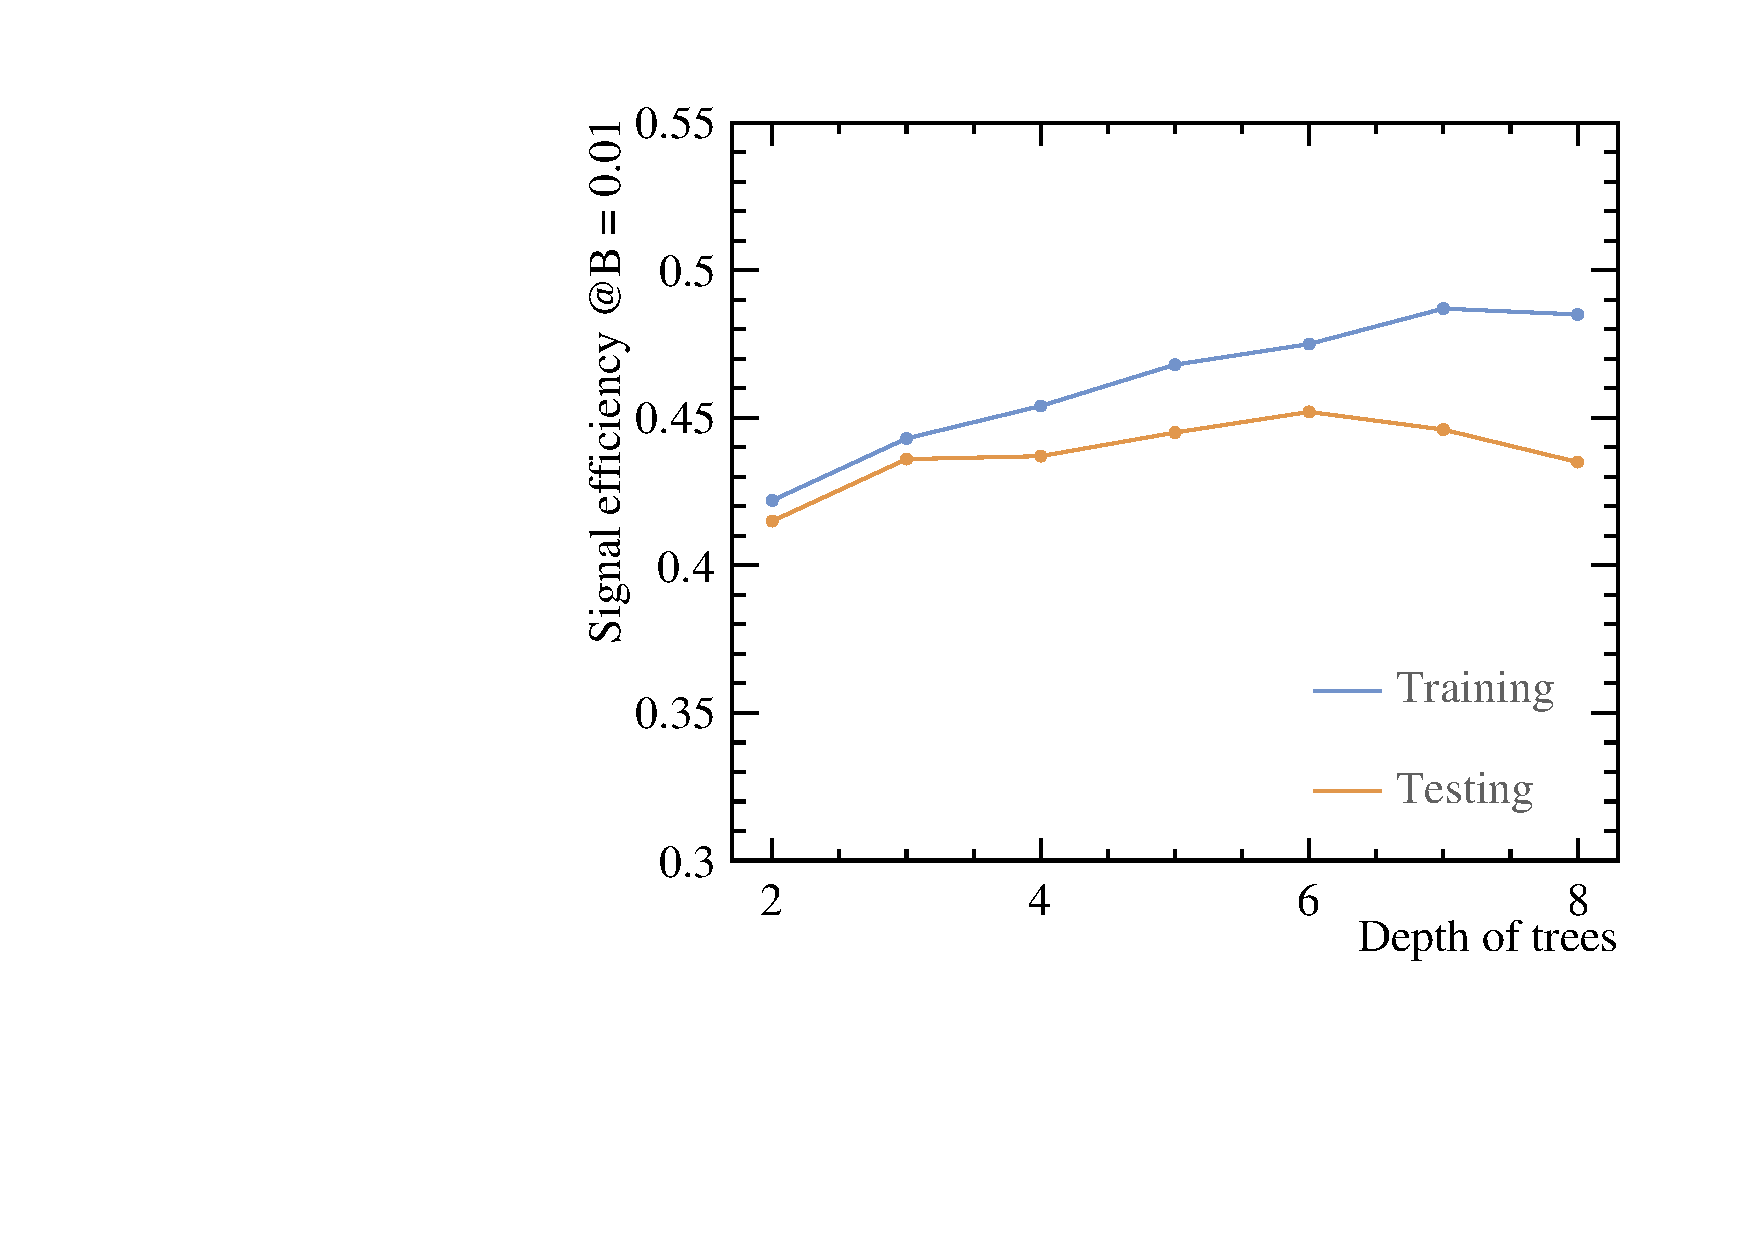
\includegraphics[width=0.85\textwidth]{doubleHiggs/DepthOfTrees.pdf}
\caption{Example of the signal selection efficiency as function of the model complexity. The example is chosen from the double Higgs analysis at \rootS{3}, using the Boosted Decision Tree model. The efficiency of the signal selection is defined as the  fraction of the signal selected when the background fraction is 1\%, reported by the TMVA training process. The depth of the tree  reflects the complexity of the model.  From a tree depth of six onwards, overfitting occurs.}
\label{fig:doubleHiggsMVAovertraining}
\end{figure}


\subsection{Choice of models}

The model to fit the data can be as simple as a cut-based model, a likelihood estimator, or a linear regression model. The model can also be as complicated as a non-linear tree, a non-linear neutral network, or a support vector machine. Regardless of the model complexity, the choice of the most optimal classifier is often data driven to match the nature of the sample. For example, a non-linear model is the best to model a non-linear response to the input variables.

To rigourously identify the best model, individual optimisation of models are required, which is computationally very expensive. However, as researchers in the machine learning suggested, the boosted decision tree is probably the best out-of-the-box machine learning method  \cite{hastie2009elements}. A neutral network model could potentially perform better than the boosted decision tree model, but it requires more tuning, and it is less intuitive to interpret. For these reasons, the boost decision tree model (BDT) is chosen for to be used in  physics analyses in this thesis. Before describing the BDT model in details, some simpler models will be described.

%the traditional rectangular cut model, and the Projective Likelihood method, which is used in the photon ID in the \pandora in \Section{}.
% often the choice of machine learning model in high energy physics. And it is
\subsection{Rectangular Cut model}

The rectangular cut method, probably the most intuitive model, optimises cuts to maximise some pre-defined metrics. The metric could be the signal efficiency for a given background efficiency. Alternatively, the metric can be the significance, $\frac{S}{\rootOf{S\!+\!B}}$, where $S$ and $B$ are respective numbers of  signal and background  passing the rectangular cuts.

Discriminative variables give better separation power when they are gaussian-like and statistically independent \cite{hastie2009elements}. Therefore it is preferable to decorrelate  the variables and gaussian transform them before using the rectangular cut MVA.

%Because of its simplicity, the cut method is often performed manually, much more often at times pre-dating the spread of machine learning methods. It is still commonly used in the analyses in  the pre-selection step before the MVA.

\subsection{Projective Likelihood model}
\label{sec:pandoraLikelihood}

The projective likelihood model with probability density estimators (PDE) is used in \pandora for the photon ID,  due to its simplicity and low requirement on computing resources. The \pandora implementation of the projective likelihood model is discussed  in \Section{sec:photonLikelihood}.
%Probability density estimators for each input variable combined in likelihood estimator (ignoring correlations

The likelihood classifier calculates the probability density for each discriminative variable, for the signal class and the  background class (hence PDE approach). The overall signal and background likelihood are defined as products of the individual probability density of each variable, for the respective signal class and background class. The likelihood ratio, $R$, can be then defined as the signal likelihood divided by the sum of the e signal likelihood and the background likelihood.

%TMVA implementation also fits an underlying function to the probability density.

%The \pandora implementation simply uses binned likelihood ratio, $R$, as the output, due to the simplicity. The sub-categories for the \pandora implementation are determined by the cluster energy.

Similar to the rectangular cut method, the likelihood model works better with decorrelated, gaussian-like variables.

%The \pandora implementation did not decorrelate nor transform the variables, to keep implementation fast.


\subsection{Decision Tree model}
\label{sec:pandoraDecisionTree}
 %is a non linear tree based model

%Before discussing boost decision tree (BDT) model, it is necessary to introduce the decision tree model.

The decision tree is a non-linear tree based model. Its rather complex nature requires a careful explanation of many concepts.

The decision tree is a binary tree, where each splitting node, the splitting point, uses a cut on a single discriminative variable to decide whether an event is signal-like (``goes down by a layer to the left''), or background-like (``goes down by a layer to the right''), depending on whether the event passes the cut. At each splitting node, samples are divided into two categories: signal-like and background-like sub-samples. For each sub-sample, this splitting process, tree growing, starts at the  root node, and stops after certain criterion are met. The root node is the first splitting node. The stopping criterion could be the minimum number of events in a node, the maximum number of layers of the tree, or a minimum/maximum signal purity of the end nodes.  The end nodes, where the tree stops growing and the sub-samples are not split, contains signal and/or background events. If there are more with more signal than background events in an end node, it is called a signal-like end node. The opposite is called a background-like end node.

%The bottom nodes that are not split are called end nodes. An end node with more signal than background events in is called a signal-like nodes. The opposite is called a background-like node.

%The two categories are then examined at splitting nodes one layer below. The tree growing starts at the root node, and stops after certain criterion are met. The stopping criterion could be the minimum number of events in a node, the maximum number of layers of the tree, or a minimum/maximum signal purity of the end nodes. The bottom nodes that are not split are called end nodes. An end node with more signal than background events in is called a signal-like nodes. The opposite is called a background-like node.

The training of the decision tree refers to finding the optimal cut at the splitting node by minimising a given metric. Assuming the probability of the cut producing the signal is $p$, three commonly used metrics for two-class classification are:
\begin{enumerate}
\item misclassification error:  $1 - \max\parenths{p\,,\,1\!-\!p}$,
\item Gini index: $2p\parenths{1\!-\!p}$,
\item cross-entropy or deviance: $-p\log{p}-\parenths{1\!-\!p}\log\parenths{1\!-\!p}$.
\end{enumerate}

The applying of a trained decision tree is performed by transversion the tree from the root node to the end node. The event is classified as signal or background, depending on whether it falls in the signal-like or background-like end node.



\FIGURE{fig:doubleHiggsMVAdecisionTree} illustrates a simple example of a trained decision tree. The signal class is the PhD student and the background class is the undergraduate student. The attributes of samples are listed \Table{tab:doubleHiggsDecisionTreeComic2}. The top diamond box,   ``Party ends before  1am'', is the root node. All diamond boxes are splitting nodes. Rectangle boxes are end nodes.  The signal-like end node is represented by the red rectangle and the background-like end nodes are represented by blue rectangles. The depth of this decision tree is two. The metric to find the optimal cut at the splinting node is the Gini index.

To demonstrate first step of the training of the model, details of finding the optimal cut at the root node are outlined. There are two possible cuts for the root node, ``Party ends before (after) 1am'' and ``(Not) Know where free pizza is''. If the cut at the root node is ``Leave party before 1am'', the probability of the cut producing the signal, $p$, is $\frac{10}{13}$, as there are 10 PhD students and 3 undergraduate students who leave parties before 1\,am. Gini index is given by
\begin{equation}
2p\parenths{1\!-\!p} \backsimeq 0.36 .
\end{equation}
If the cut at the root node is ``Know where free pizza is'', $p=\frac{10}{15}$, as there are  10 PhD students and 5 undergraduate students who know where the free pizza is located. Gini index is given by
\begin{equation}
2p\parenths{1\!-\!p} \backsimeq 0.44 .
\end{equation}
Therefore, by choosing the cut that minimise the Gini Index, the optimal cut for the root node is ``Leave party before 1am''.

The simple tree in \Figure{fig:doubleHiggsMVAdecisionTree} is grown fully as each end node contains signal or background only. An example of applying the trained decision tree is provided: if there is a student who leaves parties before 1\,am and knows where a free pizza is located, then the student is classified as a PhD student.

\begin{figure}[!htbp]
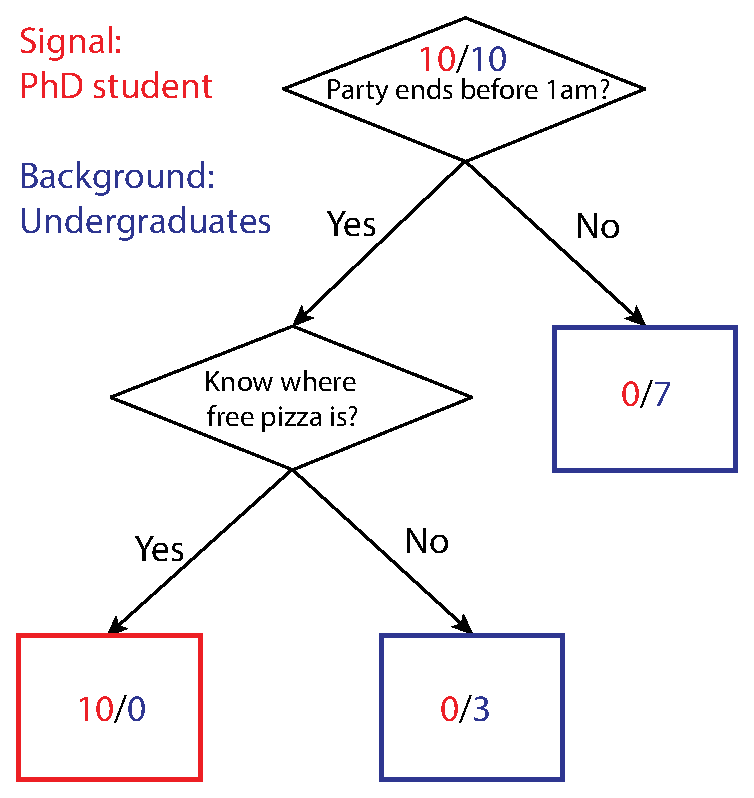
\includegraphics[width=0.65\textwidth]{doubleHiggs/mva/BDTcomic}
\caption[Example of a decision tree. ]
{Example of a decision tree. Numbers in each node represent number of PhD students (red) and number of undergraduate students (blue). Diamond boxes represent splitting nodes. Rectangular boxes represent end nodes. Blue boxes are background-like end nodes. Red boxes are signal-like end-nodes.}
   \label{fig:doubleHiggsMVAdecisionTree}
\end{figure}

\begin{table}[!htbp]\centering

\begin{tabular}{lrr}
\hline \hline
PhD students & Leave party before 1\,am  & Leave party after 1\,am\\
\hline
Know where free pizza is & 10 & 0 \\
Not know where free pizza is & 0 & 0 \\
\hline
Undergraduates & Leave party before 1\,am  & Leave party after 1\,am\\
\hline
Know where free pizza is & 0 & 5 \\
Not know where free pizza is & 3 & 2 \\
\hline \hline
\end{tabular}
\caption
{The attributes of  the PhD students and undergraduate students for the decision tree example shown in \Figure{fig:doubleHiggsMVAdecisionTree}.}
\label{tab:doubleHiggsDecisionTreeComic2}
\end{table}


\subsubsection{To improve decision tree}

%The decision tree model has a low bias, but a high variance.

%This means

It is very easy to construct a decision tree that fits the training data very well, but the tree would not be optimal for the testing sample. To overcome the instability of the decision tree model, many methods have been developed. Some of the most successful ones are boosting, bagging, and random forest.

Boosting: the basic idea of boosting is that the tree growing procedure focuses on events which are difficult to classify correctly. By assigning a weight to each event,   after each tree growing iteration, the weights for misclassified events are gradually increased. Therefore misclassified events get more attention in the next iteration.

%it is a technique where the misclassified events receives a higher weight than the correctly classified events, which makes the misclassified events more important in the training. Therefore, when the training is iterated, the misclassified events would receive higher and higher weights and be more likely to be classified correctly. The boosting can be done at every iteration. After  a few hundred or a few thousand times of iterations of training, a ``forest'' of many trees is created. The final classification could be a majority vote of the outputs of the trees, by transversing the event to the end node for each tree in the forest.

%The basic idea of adaptive boosting is that the tree making procedure focuses on events which are difficult to classify correctly. By assigning a weight to each event,   after each tree growing iteration, the weights for misclassified events are gradually increased. Therefore misclassified events get more attention in the next iteration.

Bagging: also known as boot-strap, it is a method that select a  random subset of the training sample, and use the subset at training.

%When bagging is combined with boosting, every iteration takes a subset of the  sample, rather than the whole sample.

Random Forest: when a tree is grown, a randomly selected subset of discriminative variables are used to grow the tree. %This method is know to reduce the variance of the tree.

\subsection{Boosted Decision Tree model}
\label{sec:analysisBDT}

Boosted decision tree (BDT) contains a forest of decision trees, where the boosting is used to grow trees. There are two common boosting methods: adaptive boosting and gradient boosting. The adaptive boosting,  first introduced in \cite{FREUND1997119}, is discussed in further details, as it is simpler to understand than the gradient boosting. The adaptive boosting algorithm, adapted from \cite{hastie2009elements},  is outlined below:

%where each tree is iterated many times using a technique called boosting.   By overcoming the instability of a single  decision tree, BDT is often regarded as  the best out-of-the-box machine learning method.
%The basic idea of adaptive boosting is that the tree making procedure focuses on events which are difficult to classify correctly. By assigning a weight to each event,   after each tree growing iteration, the weights for misclassified events are gradually increased. Therefore misclassified events get more attention in the next iteration.
\begin{itemize}
  \item At the initialisation stage,  event weight is initialised to $w = 1 / N$ for every event, for $N$ total events.
  \item Iterate $M$ times, where $M$ is the total number of trees. For iteration $m$:
    \begin{itemize}
      \item Create/grow a $m^{th}$ tree  with weighted samples obtained from $(m-1)^{th}$ iteration.
      \item Update $m^{th}$ tree error function, $err_m = \frac{\sum_{i = 1}^{N} w_{i,m-1} B_{i,m} }{\sum_{i = 1}^{N}w_{i,m-1}}$.
      %, where $B_{i,m} = 1$ if $i^{th}$ event is misclassified, 0 if $i^{th}$ event is correctly classified. $w_{i,m-1}$ is the event weight for $i^th$ event generated in previous iteration.
      \item Update $m^{th}$ tree weight,  $\alpha_m = \log\parenths{\frac{1 - err_m}{err_m}}$
      \item Update $i^{th}$ event weight in $m^{th}$ tree, $w_{i,m} = w_{i,m-1} e^{\alpha_m B_{i,m} }$.
    \end{itemize}
  \item The output, $G(x)$, for a testing event $x$, is a weighted vote from all M trees:
  \begin{equation}
    G(x)=
     \begin{cases}
      -1, & \mbox{if} \sum_{m=1}^{M}\alpha_mG_m(x) < 0 , \\
      1, & \mbox{otherwise}.
    \end{cases}
  \end{equation}
\end{itemize}
The tree classifier output, $G$, is denoted as  -1 or 1. One can think of -1 as background and 1 as signal. There are $N$ events and $M$ iterations (trees). The parameter $B$ represents if an event is misclassified. For the $i^{th}$ event in the  $m^{th}$ tree,  $B_{i,m} = 1$ if the event is misclassified, or 0 if the event is correctly classified. The parameter $w_{i,m}$ represent the event weight for $i^{th}$ event  in $m^{th}$ tree.


In each iteration, if the $i^{th}$ event is misclassified, the event weight increases by a factor of $(1 - err_m)/(err_m)$. Otherwise, the event weight does not change.

The power of the adaptive boosting  is to dramatically improve the performance of a weak classifier. A weak classifier is a classifier which is gives a predictive performance sightly better than a random guessing. A decision tree with a few layer would be a weak classifier. By sequentially applying many weak classifiers with weighted samples, the final ``forest'' is very robust with a very good performance.

%A weak classifier is one whose error rate is only slightly better than random guessing. The purpose of boosting is to sequentially apply the weak classification algorithm to repeatedly modified versions of the data,

%TMVA implementation of the BDT for the output uses a likelihood estimator, where the likelihood depends on how often an event is classified as signal in the forest. The likelihood number is later used to select signal from background.

\subsubsection{Optimisation of Boosted Decision Tree}
\label{sec:pandoraMVAbdtVar}

%Many parameters of the BDT can be optimised.

The most important parameter is the depth of a tree, which determines how many end nodes the tree has. It also affects the complexity of the BDT model. If the depth of a tree is set to a large value, it could leads to the overfitting of the model.
%or the degrees of freedom of the tree.

The number of trees is another important parameter. Past studies show that using many small trees yields the best result \cite{hastie2009elements}. However, intuitively a large number of trees leads to overfitting. But it has been shown that a large number does not lead to overfitting \cite{hastie2009elements}. Therefore there is a debate on the metric to determine the optimal number of trees.

The minimum number of events in a node, which is a stopping criteria for tree growing, affects the size of the tree. But it is less influential than the depth of the tree paramter.

The boosting algorithm has two variants in TMVA implementation: adaptive boost and gradient boost.

The learning rate of the adaptive boost  controls how fast the event weight changes in each boosting iteration. Studies show that a small learning rate ($\thicksim$0.1) with many trees works better than a large learning rate with fewer trees \cite{hastie2009elements}.

The shrinkage rate in the gradient boost is similar to the learning rate parameter in the adaptive boost. The shrinkage rate controls how fast the weight changes for events in each boosting iteration. Again a small value   ($\thicksim$0.1) is preferable \cite{hastie2009elements}.

The usual choice of the metric to optimise cuts for tree growing is either the Gini index or the cross-entropy. The two different metrics make  little differences to model performances.

%The use of the Gini Index  makes little differences to performances, comparing to the cross-entropy metric.
%Typically the Gini index metric is chosen.


The number of bins per variable is  a necessary parameter to make tree growing efficient, because discretely binned variables are faster to compute than continuous variables. This parameter, however,  has little  impact on the model performance. But because variables are binned, variables should be pre-processed before feeding into the training model. For example, the variable should be limited to a range to avoid the extreme values that distort the variable distribution. If the original distribution of the variable is highly skewed, the variable should be transformed to obtain a more uniform distribution.

For the end node, the output can be either signal-like or background-like, based on the majority of the training events in the end node. Numerically, it can correspond to 1/0. However, the end node could also use signal purity as the output, resulting in a continues spectrum of [0,1].

The bagging fraction determines the fraction of randomly selected samples used in each boosting iteration. By choosing a small value, samples between each boosting iteration are less correlated. Hence the overall model performance improves.

The DoPreSelection flag allows the classifier to discard phase spaces where there are only background events.

\subsection{Multiple classes}
\label{sec:pandoraMVAmulticlass}
% ATTN used in tau chapter

The above discussion  assumes two classes, the signal class and the background class. The classification can be extended to multiple classes. There are two ways for the training multiple classes. ``One versus one'' scheme trains each class against each other class. The second way is called ``one versus all'', when each class is trained against all other classes combined.
%, and the overall outputs are normalised.

Using a three-class example, A, B, and C class, ``one versus one" scheme trains A class against B class; B class against C class; and C class against A class.  ``One versus all" scheme would train A class against non-A classes; B class against non-B classes; and C class against non-C classes.

%Then the likelihood is normalised.as the background as the signa

TMVA multiple class implementation, \multiclass, uses the ``one versus all" scheme. For each class, the \multiclass classifier will train the class against all other classes. This process is repeated for each class, resulting in multiple classifiers. The overall classifier output for a single event is a normalised response using all trained classifiers, where the sum of the classifier outputs for a single event is one. Individual response of a trained classifier for an event can be treated as the likelihood. In the applying stage, the event is classified into a class if the classifier for that class gives the highest output response amongst all classifiers for that event.

The advantage of using the \multiclass classifier instead of a two-class classifier for samples with multiple classes  is the classifier outputs are correctly adjusted for multiple classes. Hence one event can  be unambiguously classified into only one class. The issue with the \multiclass classifier is that powerful discriminative variables for each individual class need to enter the training stage simultaneously, resulting in a large number of discriminative variables in the  \multiclass classifier.

%that the correlation between different classes are accounted for.
%TMVA \multiclass implementation uses "one versus all" scheme. \Multiclass is used in flavour tagging of jets, \Section{sec:pandoraLCFI}, and in the tau lepton final state separation study, \Section{}.

%Computational intensive jobs are processed either on the Cambridge High Energy Physics grid, or the \CLIC computing grid.
%Thanks computing resources. i.e. ILC VO, CLIC grid, etc. 